\documentclass[a4paper,12pt]{report}
\usepackage[utf8]{inputenc}
\usepackage{amsmath}
\usepackage{graphicx}
\usepackage{listings}
\usepackage{tikz}
\usepackage[T1]{fontenc}
\usepackage{color}
\usetikzlibrary{arrows,automata}
\definecolor{pythonred}{rgb}{0.6,0,0} % for strings
\definecolor{pythongreen}{rgb}{0.25,0.5,0.35} % comments
\definecolor{pythonpurple}{rgb}{0.5,0,0.35} % keywords
	\definecolor{pythondocblue}{rgb}{0.25,0.35,0.75} % javadoc
	 
	\lstset{language=python,
	basicstyle=\ttfamily,
	keywordstyle=\color{pythonpurple}\bfseries,
	stringstyle=\color{pythonred},
	commentstyle=\color{pythongreen},
	morecomment=[s][\color{pythondocblue}]{/**}{*/},
	numbers=left,
	numberstyle=\tiny\color{black},
        stepnumber=2,
	numbersep=10pt,
	tabsize=4,
	showspaces=false,
	showstringspaces=false}

% Title Page

 \title{\bfseries\huge \textcolor{purple}{\underline {EEP702-Software Lab}} \\{\textcolor{blue}{Assignment 4 : Program in C++/ Java for Library Management.}}}
\author{\bfseries\large\textcolor{black}  {Harshit Kumar Gupta}\\ {\textcolor{black} {2013EET2369 }}\\

\includegraphics[width=3cm,height=3.4cm]{./iit.png}\\\noindent Computer Technology\\
\noindent Department Of Electrical Engineering\\IIT DELHI}
% iit.png: 282x282 pixel, 72dpi, 9.95x9.95 cm, bb=0 0 282 282
\begin{document}
\maketitle
\tableofcontents


\chapter{\textcolor{blue}{\underline {PROBLEM STATEMENT}}}
\noindent Write a program in C++/ Java only for Library Management.
\begin{enumerate}
 \item   Use a text file to store the following information about the books available in the library.
         (Title of the book) (Author name) (Publication) (Edition)
         Read from the file and store them as array of objects. Provide user the functionality to
         search for some books based on Book title, author name, publication or any combination of these.
 \item   Add the Library Incharge Login functionality to above program which enables him to add
         or remove any book from the library. The changes must be reflected in the Library record
         and all student accounts as well.
         
  \item  Add the Student Login functionality to above program to keep a record of the books
         issued to each student along with the date of issue.
         
  \item  Add the functionality to above program to calculate total fine imposed in case any user
         fails to deposit the issued book within a period of 1 week  

\begin{center}
\chapter{\textcolor{blue}{\underline {ABSTRACT}}}
\end{center}
\noindent The Intention of the C++ Code is to make use of the Obzect oriented Approach to accomplish the task of Designing a Program which
	  interfaces with an user to add , delete or view the books which are available in a library.The Approach is rather clear where the instance
	  of a class having all the details about a book are saved and invoked from a file to be presented to a user.There are Several other privileges provided 
	  to the user depending on the status of the user , whether being a student or an admin.
\begin{center}
\chapter{\textcolor{blue}{\underline {INTRODUCTION}}}
\end{center}
\noindent C++ (pronounced see plus plus) is a programming language that is general purpose, statically typed, free-form, multi-paradigm and compiled. It is regarded as an intermediate-level language, as it comprises both high-level and low-level language features. Developed by Bjarne Stroustrup starting in 1979 at Bell Labs, C++ was originally named C with Classes, adding object-oriented features, such as classes, and other enhancements to the C programming language. The language was renamed C++ in 1983, as a pun involving the increment operator.

C++ is one of the most popular programming languages and is implemented on a wide variety of hardware and operating system platforms. As an efficient compiler to native code, its application domains include systems software, application software, device drivers, embedded software, high-performance server and client applications, and entertainment software such as video games. Several groups provide both free and proprietary C++ compiler software, including the GNU Project, LLVM, Microsoft and Intel. C++ has greatly influenced many other popular programming languages, most notably C and Java.

The language began as enhancements to C, first adding classes, then virtual functions, operator overloading, multiple inheritance, templates and exception handling, among other features. After years of development, the C++ programming language standard was ratified in 1998 as ISO/IEC 14882:1998. The standard was amended by the 2003 technical corrigendum, ISO/IEC 14882:2003. The current standard extending C++ with new features was ratified and published by ISO in September 2011 as ISO/IEC 14882:2011 (informally known as C++11).

\begin{center}
\chapter{\textcolor{blue}{\underline {SPECIFICATIONS AND ASSUMPTIONS}}}
\end{center}
\section*{Specifications}

\begin{enumerate}
\item Different Functions have been used for different obzectives.
\item show function is used to display the books available
\item book Edition has been acted as a unique value with the book name to identify a book
\item student privileges are only limited to view and add books.
\item admin , faculty login can delete the books as required.
\item atoi function has been invoked from stdlib Library.

\end{enumerate}

\section*{Assumptions}

\begin{enumerate}
\item There are as such no multiple copies of a book for same edition.
\item The author name and other such variables accept character Values only.
\item Error handling has been done accordingly for non existent books or as such .

\end{enumerate}
 
\begin{center}
\chapter{\textcolor{blue}{\underline {LOGIC USED/METHODOLOGY}}}
\end{center}
The methodology that is used for developing the program is defined below:\\

\begin{enumerate}
\item Basically , We intiate our code in C++ with the switch case command.
\item They avail the user to use as many options they can exercise.
\item The values of the Book attributes are saved in Character only.
\item We simply create functions for all the options.
\item The class obzect of the bookk is invoked by the class instance.
\item The values are recorded intoo a file system.
\item further Searching of the values done from the file named file.txt
\item Records may be deleted added as per specification.

\end{enumerate}

\begin{center}
\chapter{\textcolor{blue}{\underline {FLOWCHART}}}
\end{center}
\noindent \\Flowchart
\begin{center}
 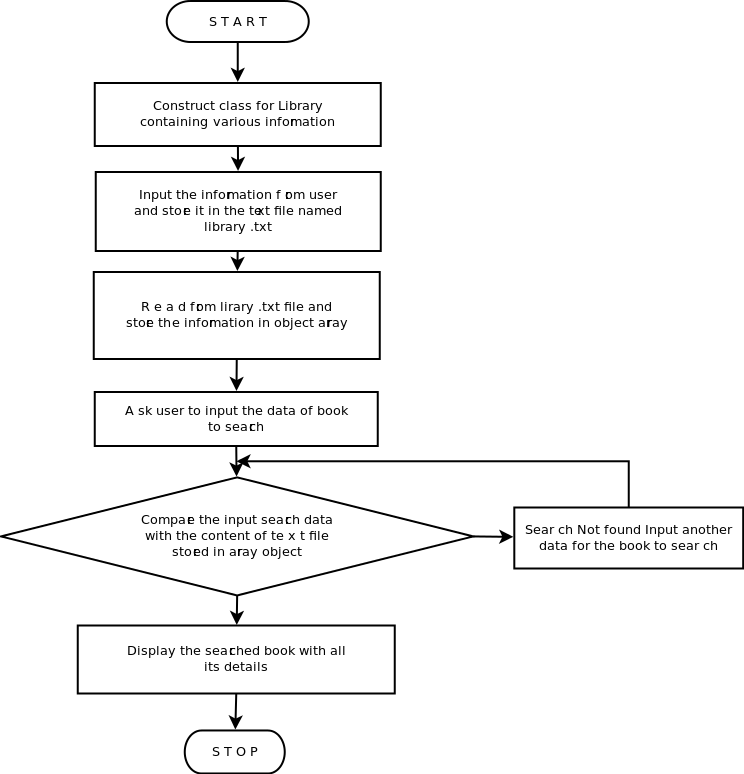
\includegraphics[width=12 cm,height=11 cm]{./flowchart.png}
 % flowchart.png: 744x774 pixel, 72dpi, 26.25x27.31 cm, bb=0 0 744 774
\end{center}

\begin{center}
\chapter{\textcolor{blue}{\underline {EXECUTION INSTRUCTIONS}}}
\end{center}
\begin{enumerate}
 \item For program following instructions are used.
 \begin{enumerate}
  \item java library.java
 \end{enumerate}

\end{enumerate}
Repeat the above instructions for different inputs.

\begin{center}
\chapter{\textcolor{blue}{\underline {RESULTS AND CONCLUSIONS}}}
\end{center}
\noindent For the given set of inputs the program exactly displays the Library management Database.\\
\begin{center}
 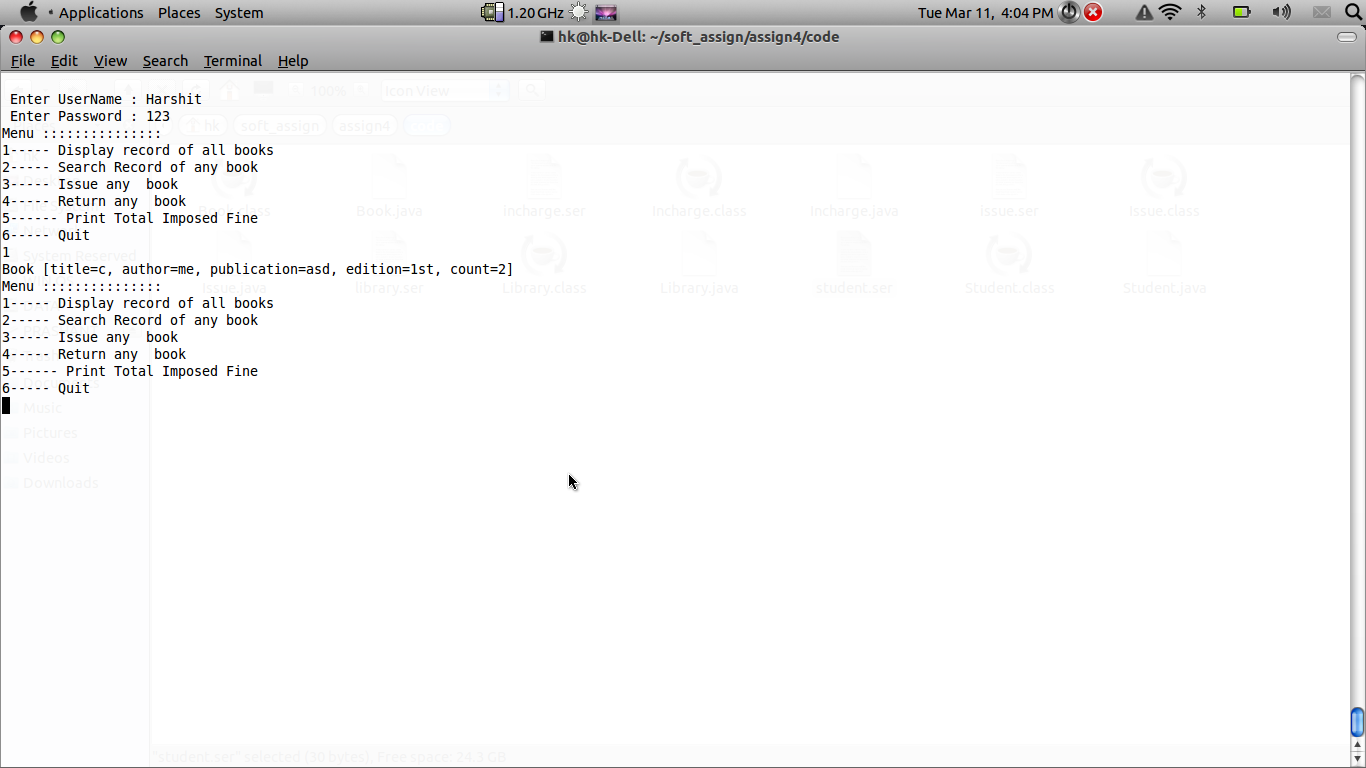
\includegraphics[width=13 cm,height=13 cm]{./output.png}
 % Output.png: 1280x800 pixel, 72dpi, 45.16x28.22 cm, bb=0 0 1280 800
\end{center}
\end{document}  
